%latex model.tex
%bibtex model
%latex model.tex
%latex model.tex
%pdflatex model.tex

%se poate lucra si online (de ex www.overleaf.com)


\documentclass[runningheads,a4paper,11pt]{report}

\usepackage{algorithmic}
\usepackage{algorithm} 
\usepackage{array}
\usepackage{amsmath}
\usepackage{amsfonts}
\usepackage{amssymb}
\usepackage{amsthm}
\usepackage{caption}
\usepackage{comment} 
\usepackage{epsfig} 
\usepackage{fancyhdr}
\usepackage[T1]{fontenc}
\usepackage{geometry} 
\usepackage{graphicx}
\usepackage[colorlinks]{hyperref} 
\usepackage[latin1]{inputenc}
\usepackage{multicol}
\usepackage{multirow} 
\usepackage{rotating}
\usepackage{setspace}
\usepackage{subfigure}
\usepackage{url}
\usepackage{verbatim}
\usepackage{xcolor}
\graphicspath{ {./images/} }

\pagestyle{fancy}
\fancyhf{}
\fancyhead[LE,RO]{ALL blood cell classification using federated learning}
\fancyfoot[RE,LO]{ITSG 2023-2024}
\fancyfoot[LE,RO]{\thepage}

\renewcommand{\headrulewidth}{2pt}
\renewcommand{\footrulewidth}{1pt}
\renewcommand{\headrule}{\hbox to\headwidth{%
  \color{lime}\leaders\hrule height \headrulewidth\hfill}}
\renewcommand{\footrule}{\hbox to\headwidth{%
  \color{lime}\leaders\hrule height \footrulewidth\hfill}}

\hypersetup{
pdftitle={artTitle},
pdfauthor={name},
pdfkeywords={pdf, latex, tex, ps2pdf, dvipdfm, pdflatex},
bookmarksnumbered,
pdfstartview={FitH},
urlcolor=cyan,
colorlinks=true,
linkcolor=red,
citecolor=green,
}


\setcounter{secnumdepth}{3}
\setcounter{tocdepth}{3}
\linespread{1}
\makeindex


\begin{document}

\begin{titlepage}
\sloppy

\begin{center}
BABE\c S BOLYAI UNIVERSITY, CLUJ NAPOCA, ROM\^ ANIA

FACULTY OF MATHEMATICS AND COMPUTER SCIENCE

\vspace{6cm}

\Huge \textbf{Acute Lymphoblastic Leukemia blood cell classification using federated learning}

\vspace{1cm}

\normalsize -- ITSG report --

\end{center}


\vspace{5cm}

\begin{flushright}
Muntean Andrei, Data Science, andrei.muntean@stud.ubbcluj.ro \\
Chiorean Alexandra, Data Science, maria.alexandra.chiorean@stud.ubbcluj.ro
\end{flushright}

\vspace{1cm}

\begin{center}
2023-2024
\end{center}

\end{titlepage}

\pagenumbering{gobble}

\begin{abstract}
This project addresses the problem of early blood cell cancer detection by leveraging artificial intelligence (AI) systems for social good. Blood cancer diagnoses are inherently complex, often requiring the collaboration of multiple doctors. To tackle this, we've implemented (AI), specifically utilising the MobileNetV2\cite{sandler2018mobilenetv2}  model, to analyse microscopic images of blood cells. To ensure the privacy of the patients while also improving our AI we've tried a pioneering approach known as federated learning. This methodology allows the AI to learn from diverse data sources in various hospitals without compromising privacy. Our project has yielded promising results, particularly with the MobileNetV2\cite{sandler2018mobilenetv2}  model, which has surpassed initial expectations. Additionally, we've developed a user-friendly web tool, streamlining the integration of our system into the testing procedures of medical professionals. However, there are a lot of challenges with the federated learning approach, notably the limitation of computing power  which lead us to rely on Google Colab with its own set of limitations.

\end{abstract}


\tableofcontents

\newpage

\listoftables
\listoffigures

\newpage

\setstretch{1.5}



\newpage

\pagenumbering{arabic}


 


\chapter{Introduction}
\label{chapter:introduction}

\section{What? Why? How?}
\label{section:what}

In US, approximately at each 3 minutes, a person is diagnosed with blood cancer. This disease is caused by the dysfunction of the bone marrow and can affect different blood types, resulting in different types of cancer like: Leukemia, lymphoma, myeloma, myelodysplastic syndromes (MDS), and myeloproliferative neoplasms (MPNs). In our project, we aim to reduce the diagnosis time by providing a computer based analysis of a microscopic image using an AI model. Moreover, to enable the model accuracy, we implement a federated learning approach, such that data does not leave the medical units.
\begin{itemize}
	\item What is the (scientific) problem? 
 Whenever it's the case for a cancer diagnosis, multiple doctors are called to give their professional opinion. The blood cell cancer is even more complex, most of the time needing different tests, which are also influenced by the stage of the cancer.  
	\item Why is it important? 
 Using peripheral blood smear (PBS) images, earlier detection of the ALL can be done, therefore more patients could be saved. Besides that, having a model that can predict the stage of the ALL, could help the doctors with a pragmatic opinion, obtaining a more precise and correct diagnosis for patients. The examination of these PBS images by laboratory users is riddled with problems such as diagnostic error because the non-specific nature of ALL signs and symptoms often leads to misdiagnosis.
	\item What is your basic approach? 
 The solution we proposed is based on a Convolutional Neural Network, which is known to obtain very accurate predictions on image tasks, having different architectures for classification tasks. In the medical field, patients confidence is really important, therefore datasets generation can be a very slow and bureaucratic. To avoid this impediment, we'll implement a federated learning approach that would speedup the entire process.
\end{itemize}



\section{Paper structure and original contribution(s)}
\label{section:structure}

The research presented in this paper advances the theory, design, and implementation of several particular models. 

The main contribution of this report is to present an intelligent algorithm for solving the problem of blood cell cancer, concretely Acute Lymphoblastic Leukemia, which is very important since more and more patients are diagnosed with it. The algorithm is able to classify the blood samples in 4 classes: Benign, Pre-B, Pro-B, early Pre-B, all three being malign.

The second contribution of this report consists of building an intuitive, easy-to-use and user friendly software application. Our aim is to build a product that would enable doctors or patients to upload an image with the PBS on our website, where the model would predict the class of the blood sample. This application can be seen as a tool for doctors when they need a second, objective opinion, but also for the patients who could find a possible interpretation of their medical test before going to a specialist.

The third contribution in this report is related to the learning procedure. Since most of the medical data is very sensitive and confidential, we aim to train our model in a Federated Learning approach, making the development and accuracy of the algorithm increase sooner. The data that the medical units is already having we'll be fed to the model, encoded, such that the data cannot be retrieved from the model. In this way, we take advantage of the quality and quantity of data, that each unit has, but it reaches to a greater purpose where patients from different location can be helped, on click away.

The first chapter is a short introduction in the blood cell cancer classification and its purpose in the current medical context.

The second chapter describes the problem in more details, having also more information about the design decision taken for implementing the software application.

The chapter \ref{chapter:stateOfArt} details briefly presents the current state of the art algorithms in both medical image classification and federated learning approaches.

The chapter \ref{chapter:proposedApproach} details the solution we are going to implement, starting from a smaller model, on which more complex layers we'll be added later. Moreover, this section will detail the necessary changes and adaptations done in order to synchronise model's learning results.

In the chapter \ref{chapter:application} an analytical analysis will be drawn. Result obtain during the training process and a comparison with SOTA, and also describing the methodology of obtaining them should be documented.

Chapter \ref{chapter:swot} will describe the strengths, the opportunities, threads and weaknesses of our algorithm, as well as of our software application.

Finally, a conclusion chapter will be summarizing our results, future plans, why and how our approach is helping the society around us.

\section{Analyzing the philosophical aspects}
\label{section:philosophicalAspects}

This application has the potential to save lives by detecting Acute Lymphoblastic Leukemia early. Early detection can lead to more effective treatment and improved outcomes for patients. Not only that, but this application can make diagnosis simpler and more accessible, as it can also be used in communities without trained professionals for pre-scanning. However, if the model is not accurate enough, it can have false positives or negatives, and such a diagnosis can have serious consequences for patients.

A false positive can cause unnecessary stress and anxiety. Receiving a cancer diagnosis, even if it's later proven to be incorrect, can have a profound emotional impact on an individual and their loved ones. It can also put the patient under unnecessary and invasive medical procedures such as biopsies or other diagnostic tests. We should also consider the unnecessary risks these investigations have. 

A false negative  can be even more critical. The patient might not receive the necessary treatment in a timely manner, potentially allowing the cancer to progress to a more advanced stage, significantly reducing the patient's chances of being cured.

The emotional toll on an individual receiving an incorrect diagnosis can be profound. False positives may lead to unnecessary emotional distress, while false negatives might create a false sense of security that could be shattered later.

We must ensure that medical professionals are involved in the decision-making process. Transparent communication with patients about the limitations and possibilities of AI in medical diagnostics is also vital to managing expectations and reducing potential negative impacts on their lives.

Patients should be informed about the use of their data for training AI models, and their consent should be obtained to ensure transparency and respect for individual autonomy. Federated learning addresses some privacy concerns by keeping patient data within hospitals. However, it's essential to ensure that the federated learning process is secure to prevent any unauthorised access to sensitive medical information. If patient data is not properly anonymized before being used in the federated learning process, there is a risk of re-identification, carrying serious emotional and legal consequences.



Our model's objectivity in classifying blood cells is critical for reliable results. Bias in the training data or model could lead to inaccuracies and potentially harm patients. While our model can assist, the final decision and interpretation should involve medical professionals who can bring their expertise and judgement to the process. There should be a standard set of criteria for identifying leukemia cells and our algorithm should be transparent and provide the reason why it classifies something as cancer or not.

In summary, while the project has the potential to significantly benefit society by detecting leukemia early, careful attention must be paid to ethical considerations, privacy, and the objectivity of the AI model. Regular evaluations and collaboration with medical professionals can help ensure the success of the project while minimising potential risks and ethical concerns.

\chapter{Scientific Problem}
\label{section:scientificProblem}


\section{Problem definition}
\label{section:problemDefinition}

Blood cell cancers, also known as hematologic cancers primarily affect the blood, bone marrow, lymph nodes, and spleen. These cancers are classified based on the specific type of blood cell affected and whether they are acute (develop rapidly) or chronic (develop gradually). Our main focus is to identify if a patient suffers from a benign or malign  Acute Lymphoblastic Leukemia (ALL) which affects immature lymphocytes. To do this we are using a CNN which  can analyze vast amounts of medical images, to detect subtle patterns indicative of early-stage ALL. Early diagnosis often leads to more effective treatments and improved outcomes. 

CNNs excel at recognizing intricate patterns within images, even subtle ones that might be challenging for the human eye to discern. In PBS images, CNNs can identify specific cell types, anomalies, and morphological features. They can efficiently process large datasets, including thousands of PBS images, in a relatively short amount of time. This ability is essential for quick and accurate diagnosis, especially in busy clinical settings. CNNs can undergo continuous learning with new data, allowing them to adapt and improve their performance over time. As more annotated PBS images become available, CNNs can refine their algorithms, leading to enhanced accuracy in diagnosis.

However, while CNNs can outperform doctors in specific tasks related to PBS image analysis, it's important to note that these technologies are most effective when used in conjunction with medical professionals. Doctors can provide critical context, interpret complex clinical situations, and make informed decisions based on the combined analysis of imaging data, patient history, and other relevant information. The synergy between intelligent algorithms and medical expertise can lead to the most accurate and comprehensive diagnoses.

Training such a model can become a very challenging task, due to the data sensitivity. Even though hospitals are possessing it, the collecting process can be very complicate. A solution for this problem is the federated learning. This method addresses privacy concerns, allowing institutions to collaborate without sharing sensitive patient data. Local devices train models on their data, sending only model updates to a central server, reducing communication overhead and ensuring data security.

As mention before, our CNN model has an PBS image as input and it returns 4 probabilities, each for the classes available: benign, Pre-B, early Pre-B and Pro-B. The class with the heights probability, will be the result for the processed sample. The image is uploaded in our web-base application and the result is shown there, after the inference on the model is done.



\chapter{State of the art/Related work}
\label{chapter:stateOfArt}

The application development is enabled by TensorFlow, a machine learning framework which provides the backbone for building intricate neural networks and implementing the CNN model, framework that is build upon Python, a versatile and widely-used programming language. 

On the application side we use Django, a high-level Python web framework, which excels in the creation of robust and scalable web applications, providing a structured, efficient approach to backend development. 

Last but not least, we use Docker, for the federated learning process, which ensures consistency and portability, encapsulating the entire application and its dependencies within containers.

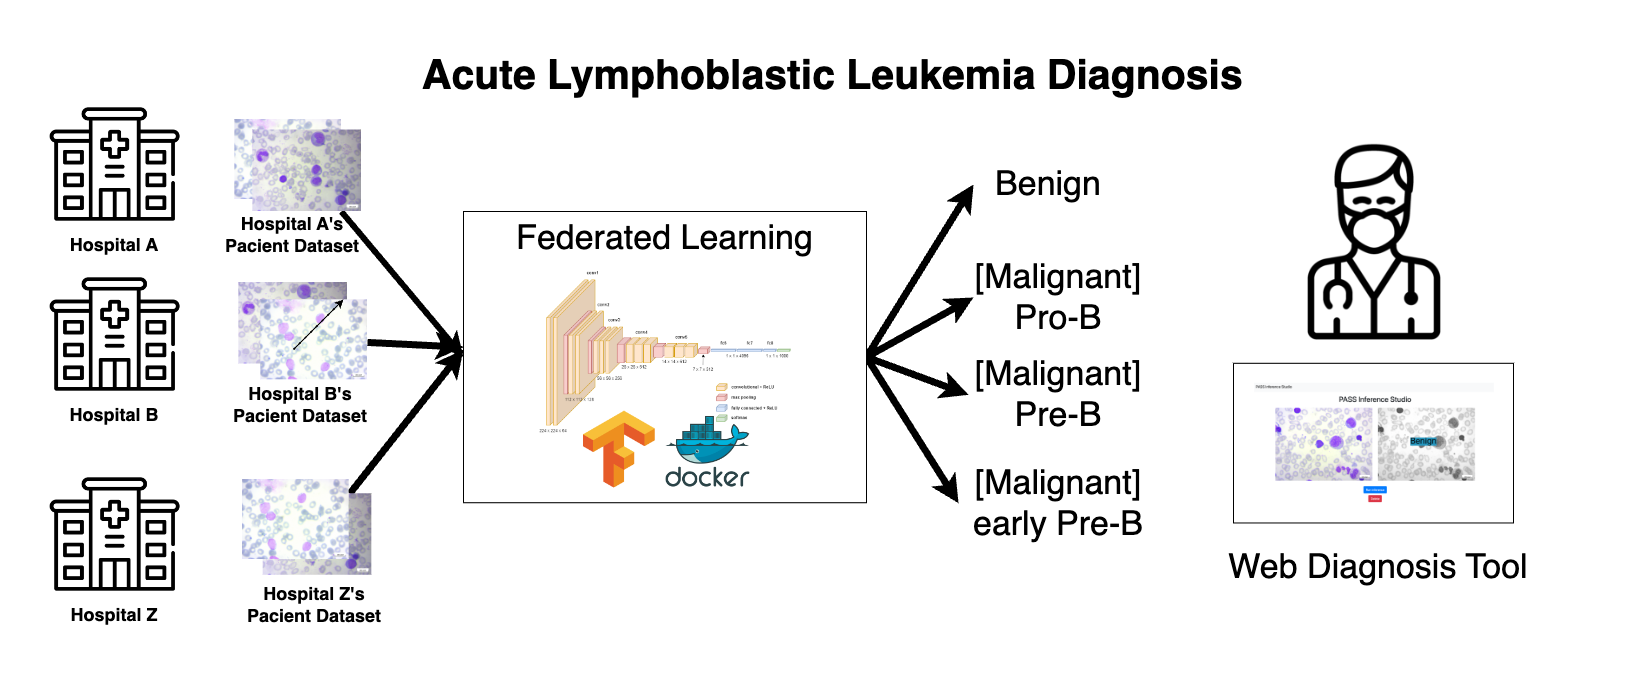
\includegraphics[scale=0.25]{images/diagram.png}


\chapter{Investigated approach}
\label{chapter:proposedApproach}

Describe in reasonable detail the algorithm you are using to address this problem. A psuedocode description of the algorithm you are using is frequently useful. Trace through a concrete example, showing how your algorithm processes this example. The example should be complex enough to illustrate all of the important aspects of the problem but simple enough to be easily understood. If possible, an intuitively meaningful example is better than one with meaningless symbols.

\section{Convolutional Neural Networks}

Convolutional Neural Networks, are a class of deep learning models specifically designed for processing images and videos. They are widely used in computer vision tasks like image recognition, object detection, and image generation. 

CNNs are able to automatically learn and extract hierarchical features from the input data. This is achieved through convolutional layers, which apply convolution operations to the input, enabling the network to detect patterns like edges, corners, and textures, making CNN very effective in medical image processing. These convolutional operations are followed by activation functions like ReLU (Rectified Linear Unit) to introduce non-linearity into the model.

\section{CNN architectures used for solving the ALL blood cell classification}
\subsection{MobileNetV2}

MobileNetV2 is an advanced deep learning architecture specifically optimized for on-device vision applications, particularly well-suited for mobile and edge devices. Developed by Google researchers, it represents an evolution of the original MobileNet model, focusing on enhancing both accuracy and efficiency in computer vision tasks.

MobileNetV2 introduces innovative features such as inverted residuals with linear bottlenecks, enabling improved gradient flow during training and maximizing computational resources. Its design includes a lightweight depthwise separable convolution followed by a linear (1x1) convolution, capturing complex patterns efficiently within a limited computational budget. Inverted residuals allow for efficient feature reuse across different layers, while depthwise separable convolutions significantly reduce parameters and computations. The model also incorporates width and resolution multipliers, offering flexibility to balance accuracy and computational efficiency. 

MobileNetV2 finds widespread application in real-time tasks like image recognition, object detection, and scene analysis on mobile devices due to its lightweight nature, making it ideal for resource-constrained environments.
\begin{figure}[h]
    \centering
    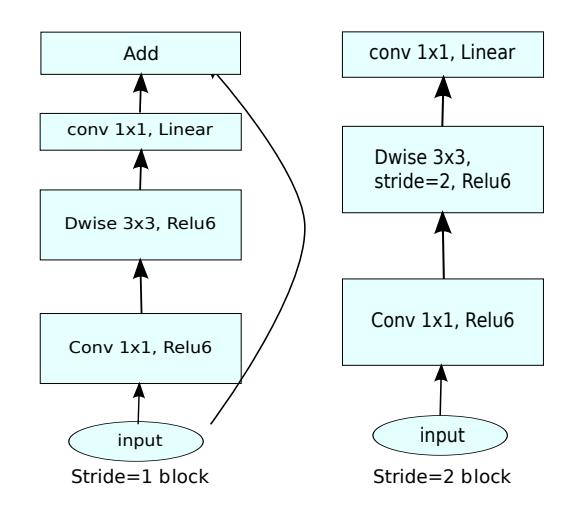
\includegraphics[scale=0.5]{images/mobilenetv2.png} 
    \caption{MobileNetV2 blocks }
\end{figure}

This backbone has approximately 3.4 million trainable parameters with 53 deep layers.
\subsection{EfficientNetB0}

EfficientNetB0 \cite{tan2019efficientnet} is the foundational model in the EfficientNet family of convolutional neural network architectures, known for its remarkable balance between accuracy and computational efficiency. Developed by Google researchers, this model leverages compound scaling to ensure that network depth, width, and resolution grow proportionally, leading to superior performance without a significant increase in computational demands. It incorporates depthwise separable convolutions for reduced parameter count and computational overhead, making it well-suited for resource-constrained devices. Regularization techniques such as dropout and batch normalization enhance its generalization and training speed. EfficientNetB0 is widely applied in various computer vision tasks, including image classification, object detection, and segmentation, and is a preferred choice for projects that require a combination of high accuracy and efficient model design.

The EfficientNetB0 has 4.01 million trainable parameters.

\subsection{MobileNet Tiny}

MobileNet Tiny \cite{howard2017mobilenets} serves as the third choice for our classification task backbone, introduced in response to the suboptimal performance of federated learning models. Derived from the groundwork laid by SSD-Lite and MobileNetV2, MobileNet-Tiny is designed to enable real-time object detection on non-GPU computers and edge devices, such as Raspberry Pi, addressing the need for efficient processing in resource-constrained environments.

\begin{figure}[h]
    \centering
    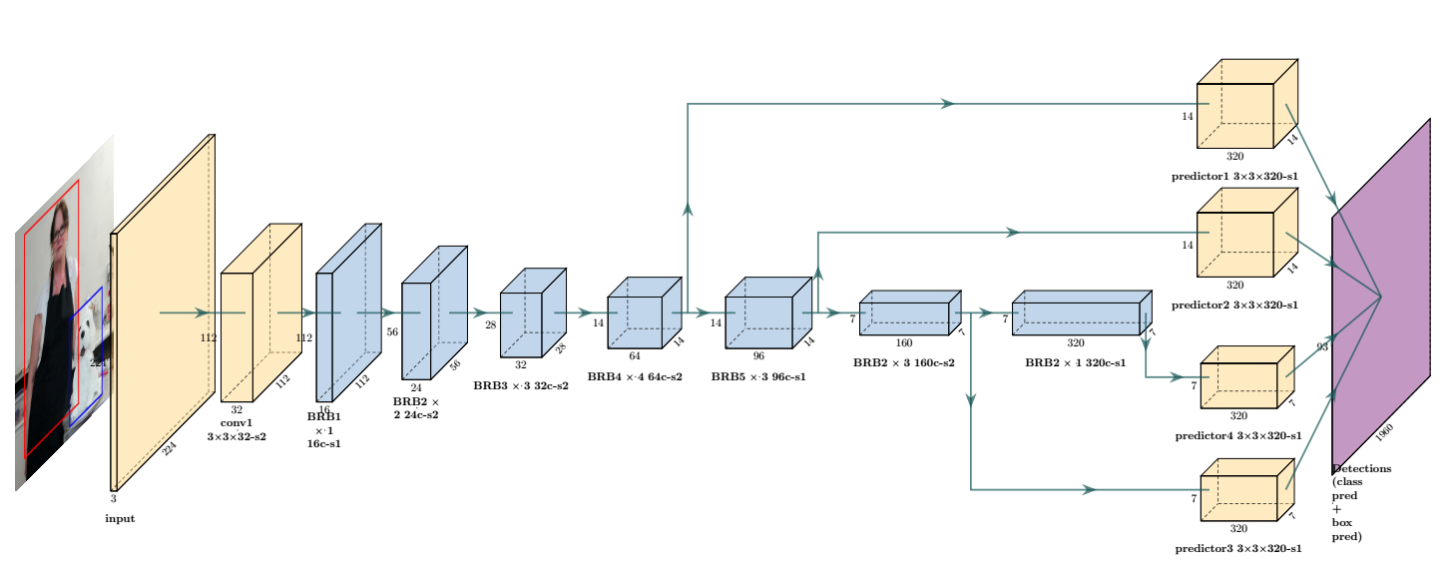
\includegraphics[scale=0.5]{images/tiny.png} 
    \caption{Tiny MobileNet}
\end{figure}

\section{Deep Learning on Decentralized Data}
Since our application processes medical data, it has a very strong privacy requirement: The patients’ data should not leave the hospital. To deal with this issue, we implement a Federated Learning approach. This enables our intelligent algorithm to learn collaboratively from multiple hospitals (edge devices) without ever sharing the sensitive data between them or with a central server. The process can be described in four phases. In the first phase, the server starts with a central model. The edge devices improve the model with their own data in phase two. In phase three, only the updates to the models are sent to the server.  Finally, the server combines the received models into a single model. The process repeats for multiple iterations which are usually just referred to as rounds.

As we have an image classification task, we will need to train a CNN in a federated way. This can pose a challenge as commonly used image classification models are quite large. We don’t expect edge devices to be very powerful, so we need to make the training process as efficient as possible. Our solution for this problem is to combine Federated Learning with Transfer Learning, meaning that we take one of the already trained image classification models (see the section above) and we freeze the backbone of the network. That means that we will only need to train the head of the network. (which we replace with a new head that can classify between our four classes). In this way we drastically reduce the number of parameters that our model has.

The development of a Federated Learning based application requires two steps: the experimentation and the deployment. In the following paragraphs we will only focus on experimentation. To experiment with federated learning, we use the dataset from Kaggle and we split it into multiple smaller datasets, one for each client. We keep this data in a different folder and we load it into a different Tensorflow Dataset, as each one of these datasets is associated with a client id. We also take into consideration that this split does not have to be equal, as in the real world some hospitals will have more data and others will have less data.

After we have split the original dataset for each client, we define the model. We use MobileNetV2 with the frozen backbone. At this step we have the model and the data, therefore we can start the federated learning simulation. For doing that, we need to initialise the weighted federated averaging algorithm. It is weighted because different weights are assigned to each client update. This is useful for giving more importance to some clients than others. To initialise this federated learning algorithm, we have to provide two optimizers. While regular training only requires a single optimizer, for federated learning we have to have two optimizers, one for the clients and one for the server.

Once the federated learning \cite{mcmahan2017communication} algorithm has been initialised, we can start the federated learning simulation. The simulation consists of multiple rounds, as explained in the first paragraph of this section. The steps are repeated for a predefined number of rounds. After the proof-of-concept has been established using the simulation, we move to the real world and try to achieve the same thing using docker. With docker compose, we define the number of clients and we mount to each client a different dataset folder. That means that now we have our data logically separated between clients, and we can test the concept in a real environment.


\chapter{Application (numerical validation)}
\label{chapter:application}

\section{Experiments with different deep models used for image classification}

Our application aims to accurately classify the four classes defining the ALL disease. To achieve this, we plan to evaluate two distinct neural networks originally designed for object recognition but adaptable for classification tasks through the addition of supplementary layers. The selected models are MobileNetV2 and EfficientNetB0. These models are suitable for the initial project prototype due to their relatively lower parameter count compared to state-of-the-art methods like VGG16, facilitating a smoother execution of the federated learning process.

Our experiments are conducted in Tensorflow, utilizing the pre-implemented versions of MobileNet and EfficientNetB0 from Keras as a starting point. We employ three different training strategies. The first involves training the model's weights from scratch using the training dataset, initialized randomly. Given our limited training samples (approximately 5,000), this method is susceptible to overfitting. The second strategy, termed fine-tuning, initializes the models with pre-trained weights from ImageNet and continues learning from that point. This approach is expected to yield superior results, leveraging the efficiency of transfer learning in classification tasks.

Finally, in an effort to further reduce the number of learnable parameters during the federated learning process, we aim to train only the last few layers of the network. This approach is anticipated to yield less favorable results due to the limited parameters and the inability to delve deeply into learning the input image.

For all training experiments the Adam optimizer is used, having the learning rate scheduler, defined by the Exponential Decay. 

\begin{figure}[h]
    \centering
    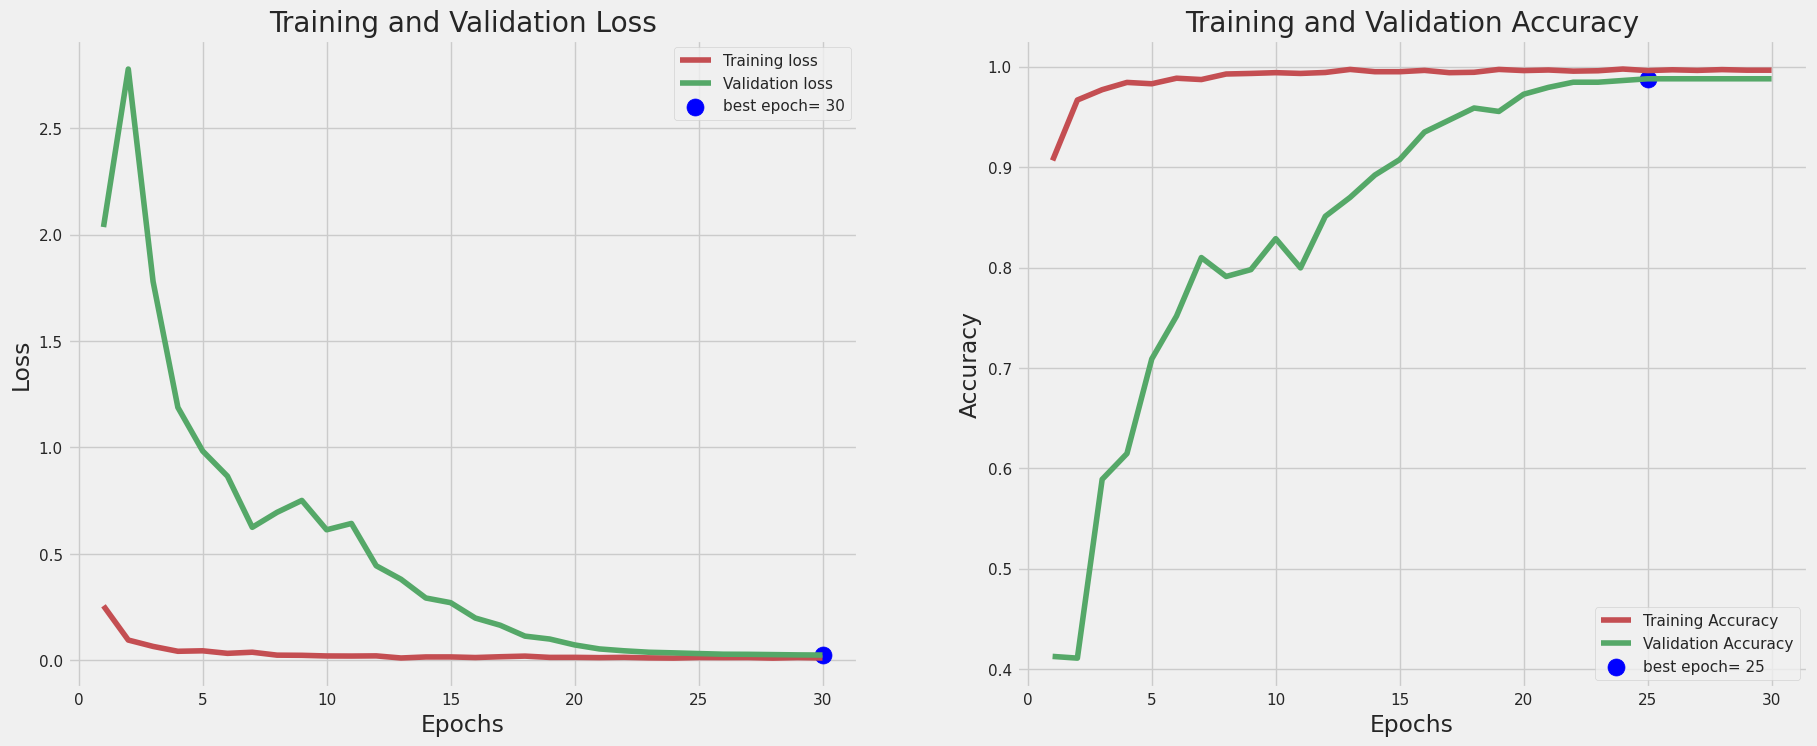
\includegraphics[scale=0.25]{images/mobilenet.png} 
    \caption{MobileNetV2 loss and accuracy values during fine-tune training }
\end{figure}

\begin{figure}[h]
    \centering
    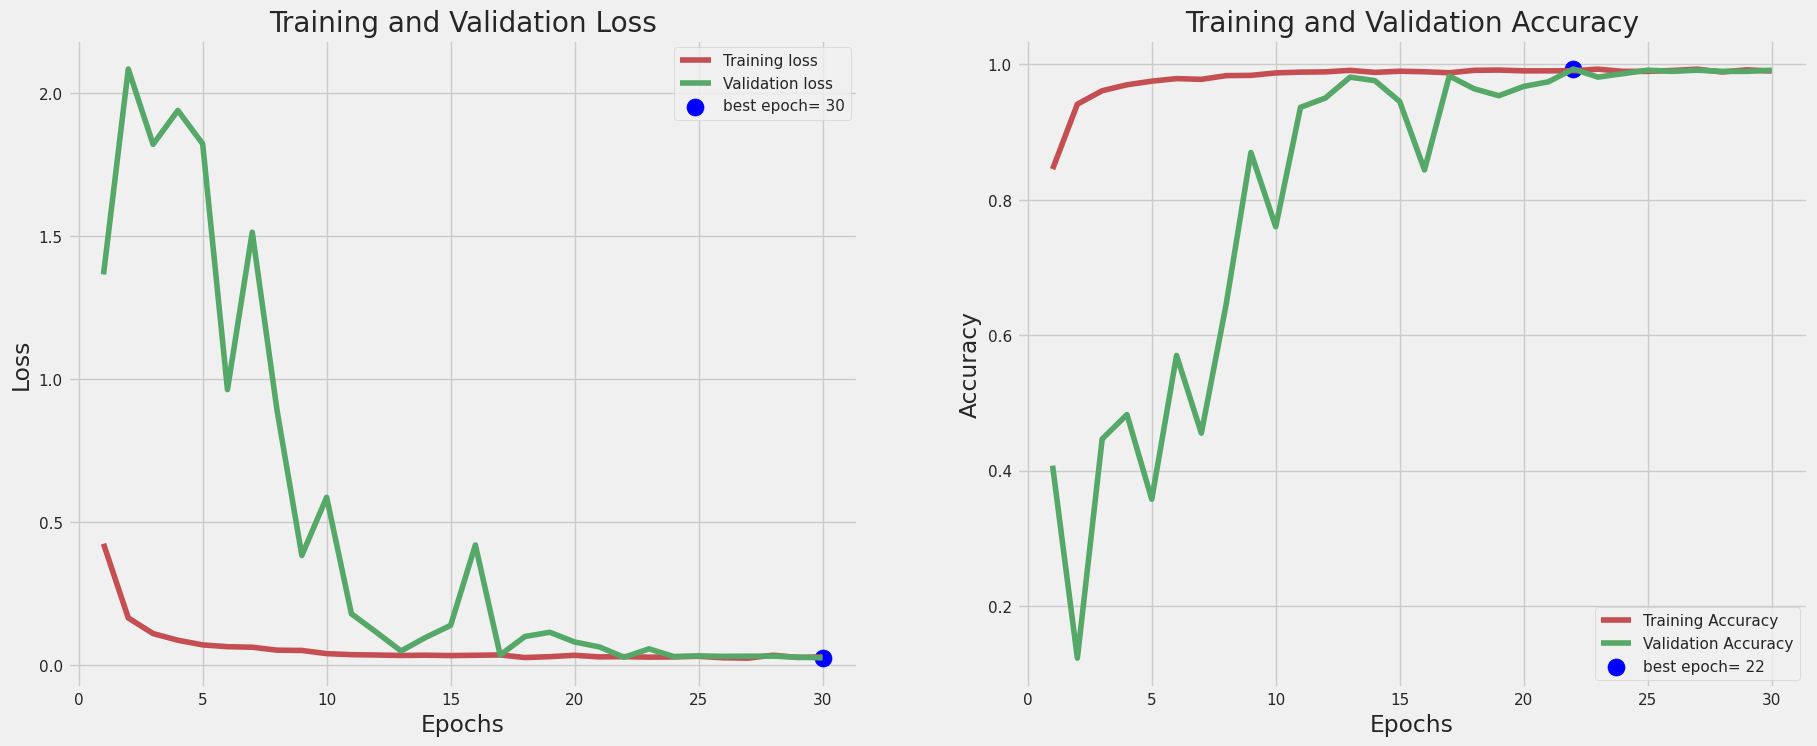
\includegraphics[scale=0.25]{images/efficientnet_plots.png} 
    \caption{EfficientNetB0 loss and accuracy values during fine-tune training }
\end{figure}


\section{Initial experiments with Federated Learning}
All federated learning experiments were performed on the MobileNetV2 model. Its architecture consists of a backbone with frozen layers, resulting in only 5716 trainable parameters. The transfer learning involved loading pretrained weights from ImageNet. The model architecture consisted of a global average pooling layer, a batch normalisation layer followed by a dense layer with softmax activation. The loss function used was sparse categorical cross entropy. With this network, the average training time for the whole dataset (3000+ training  images) was 20 minutes per round utilising a T4 GPU on Google Colab. The federated learning experiment without backbone freeze was cut short, after taking more than two hours for a single round.

In the initial experiment, a toy dataset consisting of 900 training images was used. The evaluation metrics for this experiment were sparse categorical accuracy (0.3422216) and loss (1.2883721).

Subsequent experiments involved the entire dataset, with 1458 training images for client 1 and 1459 training images for client 2. Two different optimization strategies were employed:

Experiments with Stochastic Gradient Descent Optimizer:
\begin{itemize}
\item Training setup
\begin{itemize}
    \item Backbone is freezed 
    \item Client optimizer: Stochastic Gradient Descent with Learning Rate 0.02
    \item Server optimizer: Stochastic Gradient Descent with Learning Rate 1.00
\end{itemize}
\item Experiment 1: The first experiment was done on the whole dataset, having 2 clients. We trained the model for 2 rounds, with minor  improvements in both accuracy and loss. The model seems to learn very slow. Results are summarized in table \ref{tab:results_sgd}.
\end{itemize}

\begin{table}[h!tb]
\centering
\begin{tabular}{|c|c|c|}
\hline
\textbf{Round} & \textbf{Sparse Categorical Accuracy} & \textbf{Loss} \\
\hline
1 & 0.28946334 & 1.3677657 \\
\hline
2 & 0.29013768 & 1.3658522 \\
\hline
\end{tabular}
\caption{Experiments with Stochastic Gradient Descent}
\label{tab:results_sgd}
\end{table}


Experiments with Adam Optimizer:
\begin{itemize}
\item Training setup
\begin{itemize}
    \item Backbone is freezed 
    \item Client optimizer: Adam with Learning Rate 0.0001, beta1=0.9, beta2=0.999, eps=1e-08
    \item Server optimizer: Adam with Learning Rate 0.0001, beta1=0.9, beta2=0.999, eps=1e-08
\end{itemize}

\item Experiment 1: The first experiment was done on the whole dataset, having 2 clients. We trained the model for 5 rounds, but only the first epochs gave significant improvement in both accuracy and loss. The model again seems to learn very slow. Results are summarized in table \ref{tab:results_adam}.
\end{itemize}

\begin{table}[htb]
\centering
\begin{tabular}{|c|c|c|}
\hline
\textbf{Round} & \textbf{Sparse Categorical Accuracy} & \textbf{Loss} \\
\hline
1 & 0.29784024 & 1.3651314 \\
\hline
2 & 0.2983202 & 1.3649479 \\
\hline
3 & 0.30010286 & 1.364796 \\
\hline
4 & 0.30167982 & 1.364657 \\
\hline
5 & 0.30147412 & 1.3645263 \\
\hline
\end{tabular}
\caption{Experiments with Adam Optimizer}
\label{tab:results_adam}
\end{table}

Experiments with Adam Optimizer for the client and SGD for the server:
\begin{itemize}
\item Training setup
\begin{itemize}
    \item Backbone is freezed 
    \item Client optimizer: Adam with Learning Rate 0.0001, beta1=0.9, beta2=0.999, eps=1e-08
    \item Server optimizer: Stochastic Gradient Descent with Learning Rate 1.00
\end{itemize}
\item Experiment 1: The first experiment focuses on reducing the dataset complexity, and using only two classes: Benign and Pro-B. The dataset reduces significantly this way, having 1.2k samples for training and approximately 200 samples for testing. We changed the batch size to 4. With this setup we get an accuracy of aprox. 60\% for both test and training, after 5 epochs. The same problem with the training rate persists. Results can be seen in the table \ref{tab:results_adam_experiment_2}.
\item Experiment 2: For the second experiment we took three classes: Pre-B, Pro-B and benign. Here we changed the number of clients to 3, and we kept the batch size the same. Compared with the 2 clients training, the accuracy seams to decrease by 0.04 on the training set. From this we take that having multiple clients, will not improve the results, as long as we use the same dataset for training multiple epochs. Results are summarized in the table \ref{tab:results_adam_experiment_3}
\end{itemize}


\begin{table}[htb!]
\centering
\begin{tabular}{|c|c|c|}
\hline
\textbf{Round} & \textbf{Sparse Categorical Accuracy} & \textbf{Loss} \\
\hline
1 & 0.6013214 & 0.7844671 \\
\hline
2 & 0.60169894 & 0.6759241 \\
\hline
3 & 0.60169894 & 0.67342085 \\
\hline
4 & 0.60169894 & 0.6732075 \\
\hline
5 & 0.60169894 & 0.6731787 \\
\hline
6 & 0.60169894 & 0.67317086 \\
\hline
Evaluation results & 0.66 & 0.64 \\
\hline
\end{tabular}

\caption{Experiments with only Benign vs Pro-B class}
\label{tab:results_adam_experiment_2}
\end{table} 

\begin{table}[htb!]
\centering
\begin{tabular}{|c|c|c|}
\hline
\textbf{Round} & \textbf{Sparse Categorical Accuracy} & \textbf{Loss} \\
\hline
1 & 0.8928632 & 0.33380216 \\
\hline
2 & 0.9413339 & 0.17066188 \\
\hline
3 & \approx 0.95 & \approx 0.16 \\
\hline
\end{tabular}

\caption{Experiments with only Benign vs Pro-B class and one client}
\label{tab:results_adam_experiment_4}
\end{table} 

\begin{table}[htb!]
\centering
\begin{tabular}{|c|c|c|c|}
\hline
\textbf{Number of clients} & \textbf{Round} & \textbf{Sparse Categorical Accuracy} & \textbf{Loss} \\
\hline
\multirow{3}{1em}{2} & 1  & 0.4172 & 1.358 \\
 & 2 & 0.4197 & 1.0754 \\
 &  3 & 0.4197 & 1.0718 \\
\hline
\multirow{4}{1em}{3} & 1  & 0.4124 & 1.1569 \\
 & 2 & 0.4155 & 1.0781 \\
 &  3 & 0.4155 & 1.0725 \\
& Evaluation results & 0.4801762 &  1.04286\\
\hline
\end{tabular}
\caption{Experiments with Benign, Pre-B and Pro-B class}
\label{tab:results_adam_experiment_3}
\end{table}

\section{Methodology}
\label{section:methodology}

During the training phase, the model uses categorical cross entropy as a measure of how well it is doing its task, adjusting its parameters to minimize this loss. In the evaluation phase, the accuracy metric is used to assess the overall correctness of the model's predictions on a separate dataset. The goal during training is to improve accuracy indirectly by minimizing the chosen loss function. 

Categorical cross entropy is particularly suited for scenarios where there are multiple classes, and each input belongs to one and only one class. It compares the distribution of predicted class probabilities with the true distribution (one-hot encoded), penalizing the model more when its predictions are further from the actual values.

However, for the model evaluation accuracy metric is chosen. Accuracy is a straightforward metric that measures the proportion of correctly classified instances out of the total instances. 

\begin{itemize}
	\item What specific hypotheses does your experiment test? Describe the experimental methodology that you used. 
	\item What are the dependent and independent variables? 
	\item What is the training/test data that was used, and why is it realistic or interesting? Exactly what performance data did you collect and how are you presenting and analyzing it? Comparisons to competing methods that address the same problem are particularly useful.
\end{itemize}

\section{Data}
\label{section:data}
The dataset that is used for differentiation between acute lymphoblastic leukemia blood cells and healthy cells, is taken from Kaggle, at this url location: https://www.kaggle.com/datasets/mohammadamireshraghi/blood-cell-cancer-all-4class. 
The dataset consists of 5384 samples, divided in 4 different classes: benign, early PreB, PreB and ProB, which have the following distribution.

\begin{figure}[h]
    \centering
    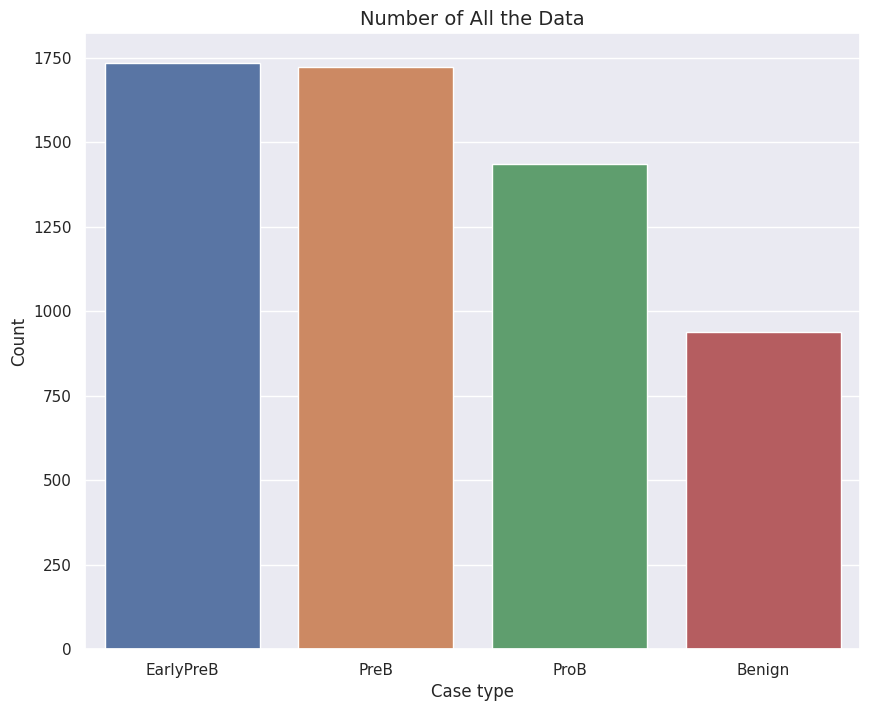
\includegraphics[scale=0.25]{images/classes_distribution.png} 
    \caption{Classes distribution in the dataset}
\end{figure}

\begin{figure}[h]
    \centering
    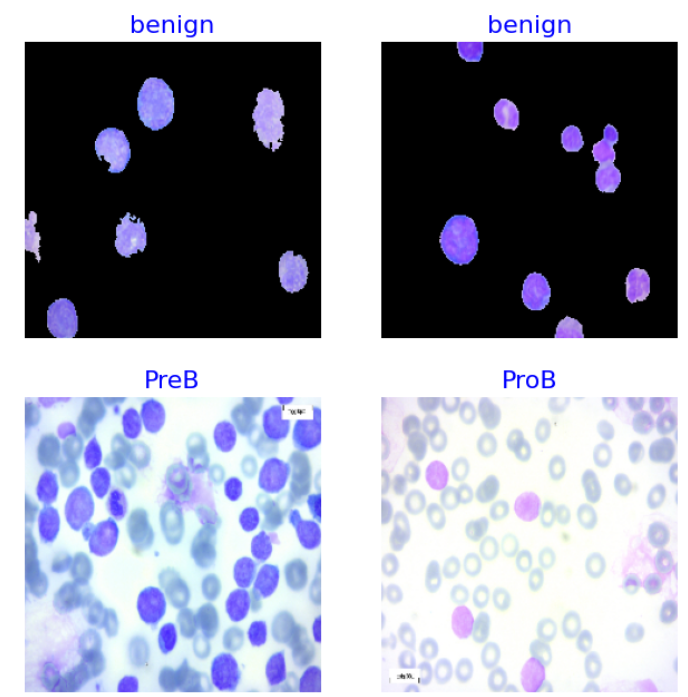
\includegraphics[scale=0.5]{images/samples.png} 
    \caption{Example of segmentation ground truth mask with correct label}
\end{figure}

To boost the training performance, augmentation is apply on the images in form of resizing, vertical and horizontal flip. The dataset is split in training, validation and test subsamples, with the ratio of 0.8 for training, 0.1 for validation and 0.1 for testing. 



\section{Results}
\label{section:results}

Below, you can find the outcomes of our initial training experiments and the accuracy of the validation step:

\begin{table}[htb]
\centering
\begin{tabular}{|c|c|c|}
\hline
\textbf{Training type} & \textbf{MobileNetv2} & \textbf{EfficientNetB0} \\
\hline
Learning from scratch & 0.30 & 0.88 \\
\hline
Fine-tune & 0.9880 & 0.9940 \\
\hline
Backbone freeze & 0.887 & 0.42 \\
\hline
\end{tabular}
\caption{Experiments of the models with different training stategies}
\label{tab:results_sgd}
\end{table}

As expected, the fine-tuning experiments are getting the best results for our classification task. The models learning curve can also be seen in the figures below. The 
small increase in the EfficentNet accuracy is due to the additional 0.6 milion parameters, but for the current use-case, we choose to go with the MobileNet even though the accuracy is slightly smaller.  

However, the results for full training and the backbone freeze are quite puzzling, We can see that EfficientNet is able to learn, without overfitting, while MobileNet hasn't learned anything. This behaviour has to be investigated in the future.

Present the quantitative results of your experiments. Graphical data presentation such as graphs and histograms are frequently better than tables. What are the basic differences revealed in the data. Are they statistically significant?


\chapter{SWOT Analysis}
\label{chapter:swot}
\section*{Strengths:}
The MobileNetV2\cite{sandler2018mobilenetv2} model has surpassed expectations in blood cell cancer classification, demonstrating remarkable performance. The user-friendly web client and seamless integration with Azure enable efficient testing and model deployment.

\section*{Weaknesses:}
Challenges arise in federated learning implementation due to limited computational resources and few data samples. Framework issues, including but not limited to obsolete packages and conflicts, made us use external Google Colab exclusively.

\section*{Opportunities:}
Expanding the dataset and regular model updates offer opportunities to improve accuracy, while exploring better workstations can address slow convergence issues, enhancing overall efficiency and system capabilities.

\section*{Threats:}
High computational demands in federated learning may limit scalability, and frequent framework issues pose a threat to system stability.

\chapter{Conclusion and future work}
\label{chapter:concl}

In conclusion, our Acute Lymphoblastic Leukaemia​ blood cell cancer classification has yielded exceptionally positive results with the MobileNetV2\cite{sandler2018mobilenetv2}  model surpassing expectations. The implementation of the federated learning approach has shown promise, although challenges arise due to limited computational resources and insufficient data. We have discovered that using federated learning in a practical way requires way better computational resources than we had available on Google Collab and it is also crucial to expand the dataset when compared to the traditional approach because otherwise the model converges more slowly.
We have also successfully developed an user-friendly web-based client for running inferences on blood samples, contributing to efficient testing procedures for the doctors involved. Because we use  the Azure cloud for storing and uploading our models we have enabled extremely short development cycles, making better models very easy to deploy to many clients.

However, it's worth noting that the federated learning framework currently utilises obsolete packages and has a lot of conflicts, making it extremely hard to train on our hardware. To overcome this challenge, we had to use the curated environment from Google Colab.

In essence, our findings highlight the potential of deep learning methods, MobileNetV2\cite{sandler2018mobilenetv2}  in particular, for blood cell cancer detection and the benefits of a federated learning approach, while emphasising the very high computational resources demanded by this new privacy-preserving technology and the need to expand the datasets. 

Looking ahead, we need to add more data sources in our dataset to increase the number of samples and to update the model regularly to make it better at classifying blood cell cancer. The new data should help the model become more accurate and reliable. Also, we should figure out ways to gain access to better workstations to speed up the learning process.


\bibliographystyle{plain}
\bibliography{BibAll}

\end{document}

